% Load the base class
\documentclass[minted, draw]{../tex/hebdomon}
\usepackage{svg}
\begin{document}

\title{Blood Cells Detection and Classification using Deep Learning and Machine Learning}
\author{v0.1}
\StudentName{Achille Cannavale}
\date{dtm@mci4me.at}

\publishers{
  \begin{tabular}[!b]{rl}
  \textbf{Student Name} & Achille Cannavale \\[3pt]
  \textbf{Student Number} & xxxxx \\[3pt]
  \textbf{Module Name} & xxxxx
  \end{tabular}\\[20pt]
  }

\begin{titlepage}
    \centering
	
\includegraphics[width=4cm]{figures/logo.png}\par\vspace{1cm}

    %\vspace*{2cm}

    {\scshape\LARGE Università degli Studi di Cassino e del Lazio Meridionale\par}
    \vspace{1cm}
    {\Large Corso di Laurea Magistrale in Ingegneria Informatica \par}

    \vspace{2cm}
    {\Huge\bfseries Blood Cells Detection and Classification using Deep Learning and Machine Learning\par}
    \vspace{1cm}
    {\large Versione 0.1}

    \vfill

    \begin{flushleft}
    \textbf{Cannavale Achille} \\
    \textbf{Colacicco Nunziamaria} \\
    \textbf{La Torre Noemi} \\
    \end{flushleft}

    \vspace{1.5cm}

    {\large \today\par}
\end{titlepage}

\dominitoc
\tableofcontents
\newpage

\Chapter{}
\Section{Introduzione}

La malaria è una delle principali malattie infettive a livello globale, con un impatto significativo sulla salute pubblica, in particolare nei paesi tropicali e subtropicali. Tra i diversi parassiti responsabili di questa patologia, il \hlight{Plasmodium vivax} rappresenta una delle specie più diffuse. La diagnosi precoce e accurata è fondamentale per un trattamento tempestivo ed efficace, e l’analisi microscopica degli strisci ematici rimane uno degli strumenti diagnostici più affidabili.
In questo progetto, viene affrontato il problema della rilevazione e classificazione automatica delle cellule del sangue infettate da P. vivax, attraverso tecniche di machine e deep learning.
Utilizzando il dataset \hlight{P. vivax malaria infected human blood smears}, che contiene oltre \textbf{1.300} immagini microscopiche annotate con più di \textbf{86.000} cellule identificate e classificate, si propone una pipeline (Figura \ref{fig:pipeline_general}) che combina \textbf{Deep Learning} e \textbf{Machine Learning} per:

\begin{itemize}
	\item individuare automaticamente le regioni di interesse (ROI) contenenti cellule
	\item estrarre le feature significative dalle ROI
	\item classificare ogni cellula in una delle categorie predefinite, tra cui cellule sane (red blood cell e leucocity) e diversi stadi del parassita infetto (trophozoite, ring, gametocyte, ecc.)
\end{itemize}

\begin{warning}
	L’analisi di questo lavoro ha evidenziato una marcata sbilanciatura del dataset, aspetto che ha richiesto un’attenta progettazione delle strategie di addestramento.
\end{warning}
%
\begin{figure}[ht]
	\centering
	\includesvg[width=\linewidth]{figures/pipeline_general.svg}
	\caption{Pipeline Generale del nostro progetto, suddivisa in una fase di Deep Learning per per la rilevazione delle ROI e l'estrazione delle features e una fase di Machine Learning per la classificazione delle cellule.}
	\label{fig:pipeline_general}
\end{figure}
%
\Section{Strumenti Utilizzati}
Per lo sviluppo del progetto, sono stati utilizzati i seguenti strumenti software:

\begin{itemize}
	\item Parte di \textbf{Deep Learning:}
	\begin{itemize}
		\item \textbf{PyTorch}: per la progettazione, addestramento e valutazione dei modelli di Deep Learning
	\end{itemize}
	\item Parte di \textbf{Machine Learning:}
	\item \textbf{Scikit-Learn}: per l’implementazione di algoritmi di Machine Learning
	\item Strumenti \textbf{Ausiliari:}
	\begin{itemize}
		\item \textbf{Numpy} e \textbf{Pandas}: per l’analisi dei dati
		\item \textbf{Matplotlib} e \textbf{Seaborn}: per la visualizzazione dei dati e dei risultati
	\end{itemize}
\end{itemize}

\section{Composizione del Dataset}
Il Dataset preso in esame è composto da 1.328 immagini e da 86.035 oggetti. Ogni oggetto può appartenere ad una delle seguenti 7 classi:
\begin{itemize}
	\item \textbf{red blood cell} (RBC): globuli rossi sani (83,034)
	\item \textbf{trophozoite}: stadio iniziale del parassita (1,584)
	\item \textbf{ring}: stadio di anello del parassita (1,617)
	\item \textbf{difficult}: stadio difficile del parassita (446)
	\item \textbf{schizont}: stadio avanzato del parassita (190)
	\item \textbf{gametocyte}: stadio gametico del parassita (156)
	\item \textbf{leukocyte}: globuli bianchi sani (103)
	
\end{itemize}


Da qui possiamo già evincere il grandissimo squilibrio presente nel dataset, rappresentato dalla classe maggioritaria delle \textbf{red blood cell}.


\Chapter{Deep Learning}

\Section{Trasformazioni}
Per garantire una buona generalizzazione del modello, sono state provate diverse trasformazioni, usando la libreria \hlight{Albumentation}, tra le quali sono state scelte le seguenti migliori per il nostro caso di studio: (anche una tabella va bene)


%
\begin{table}[!ht]
	\begin{NiceTabular}{rX}[rules/color=[gray]{0.9},rules/width=1pt]
		\CodeBefore
		\rowcolors{1}{black!5}{}
		\rowcolors{3}{blue!5}{}
		\Body
		\toprule
		\textbf{Trasformazione}      & \textbf{Parametri}                                \\
		\midrule
		\textbf{A.HorizontalFlip} & p=0.5          \\
		\textbf{A.VerticalFlip}   & p=0.5        \\
		\textbf{A.ColorJitter} & brightness=0.2, contrast=0.2, saturation=0.2, hue=0.1, p=0.3\\
		\textbf{A.RandomBrightnessContrast} & p=0.3\\
		\textbf{A.MotionBlur} & p=0.2\\
		\textbf{A.GaussNoise} & p=0.2\\
		\textbf{A.CLAHE} & p=0.2 \\
		\textbf{A.CoarseDropout} & num holes ange=(3, 6), hole height range=(10, 20), hole width range=(10, 20), fill="random uniform", p=0.2 \\
		\textbf{A.Resize} & 800x800 \\
		\textbf{A.Normalize} & mean=[0.7205, 0.7203, 0.7649], std=[0.2195, 0.2277, 0.1588] \\
		\bottomrule
	\end{NiceTabular}
	\caption{Lista delle trasformazioni utilizzate per il dataset.}
\end{table}
%


In particolare, I parametri della normalizzazione sono stati calcolati dal dataset stesso:
\begin{table}[!ht]
	\begin{NiceTabular}{rX}[rules/color=[gray]{0.9},rules/width=1pt]
		\CodeBefore
		\rowcolors{1}{black!5}{}
		\rowcolors{3}{blue!5}{}
		\Body
		\toprule
		\textbf{Parametro}      & \textbf{Valore}                                \\
		\midrule
		\textbf{Media RGB} & (0.7205, 0.7203, 0.7649) \\
		\textbf{Deviazione standard RGB} & (0.2195, 0.2277, 0.1588) \\
		\bottomrule
	\end{NiceTabular}
	\caption{Valori di media e deviazione standard per la normalizzazione delle immagini.}
\end{table}

Una delle trasformazioni che hanno garantito un forte miglioramento è rappresentata da \hlight{CoarseDropout}, che randomicamente oscura regioni rettangolari dall’immagine, simulando l’occlusione ottica e variando la grandezza degli oggetti nel mondo reale. (esempi immagine)








%
% \begin{excerpt}
% 	To see the image, have a look at Figure 1.1.
% \end{excerpt}
%

%
\Section{Defined Environments}
%
\begin{hgitemize}
	\item[\pcode{excerpt}] The template relies on the excellent \lstinline[columns=fixed]{tcolorbox}
	package for formatting the boxes within the document and for that end different styles were created.
	\item[] Sometimes one needs to quote either a proverb or to create drama, for this use
	the \lstinline[columns=fixed]{excerpt} environment with the following notation and effect.
\end{hgitemize}
%
\begin{code}{latex}
\begin{excerpt}
  To be, or not to be...
\end{excerpt}
\end{code}
%
\begin{hgitemize}
	\item[] Compiling this code snippet would show as in the document
\end{hgitemize}
%
\begin{excerpt}
	To be, or not to be...
\end{excerpt}
%
\begin{itemize}[leftmargin=!,labelindent=-29.2pt]
	\item[\pcode{code}] During the preparation of your document, it is useful to showcase
	      some code either in the shape of all the document or a snippet of it.
	      There are two (\hlight{2}) ways of doing this where the first one will be discussed here.
	\item[] For example to print out a hello world in python, please use the following environment
\end{itemize}
%
\begin{verbatim}
\begin{code}{python}
print("Hello, World!")
\end{code}
\end{verbatim}
%
Producing the following:
%
\begin{code}{python}
print("Hello, World!")
\end{code}
%
The class also come with some predefined environments to modify the behaviour/aesthetics of the document.
%
Highlighting text is \hlight{very easy}, here is an example on how to write one.

\begin{code}{latex}
Highlighting text is \hlight{very easy}, here is an example:
\end{code}

\begin{itemize}[leftmargin=!,labelindent=-29.2pt]
	\item[\pcode{example}] Sometimes you need to showcase an example or
	      need to highlight a certain idea.
	      For these things the environment Example could be useful.
	\item[] For example to show as simple example or give a slight attention to a topic you can do the following.
\end{itemize}

\begin{example}
	This is an example. This could be anything which you would like to have a certain amount of
	attention but not too much as to distract from the flow of the document.
\end{example}

\begin{itemize}[leftmargin=!,labelindent=-29.2pt]
	\item[\pcode{highlight}] Or sometimes you need to give a clear break to the flow of the
	      document and ask the reader to look at your banner. For that use highlight.
\end{itemize}

\begin{highlight}
	Hey! Pay attention as this is a highlight box.
\end{highlight}

\Subsection{Writing Equations}
%
One of the strong suits of LaTeX compared to other editors and programs is
it simplicity and ease of use methods of writing equations. Consider the
following equation:
%
\begin{equation*}
	f(x) = x^2 + 2x + 1
\end{equation*}
%
In code form this would be written as:
%
\begin{code}{latex}
	\begin{equation*}
		f(x) = x^2 + 2x + 1
	\end{equation*}
\end{code}
%
All equations that has their newline and centre staged are mostly written
in an environment where it has a \pcode{begin} and an \pcode{end}. You may
have noticed the asterisks sign just after the equation. This implies the
environment is \hlight{not numbered}, meaning you won't be able to
reference it. This is used to limit the numbering of equations to just the
essential parts in the document and not reach 3 digits by the time you are
in page 8. For a numbered equation like the following
%
\begin{equation}
	f(x) = x^2 + 2x + 1
\end{equation}
%
You only need to do:
%
\begin{code}{latex}
	\begin{equation}\label{eq:quad}
		f(x) = x^2 + 2x + 1
	\end{equation}
\end{code}
% 
where \pcode{\label{eq:quad}} is the equation reference label.
%
You could also make matrices as well as \pcode{amsmath} is preloaded into this template.
%
\Subsection{Designing a Table}
%
Finally, no template is done without someone telling you how a table should be designed.
%
Below is a standard table
%
\begin{table}[!ht]
	\begin{NiceTabular}{rX}[rules/color=[gray]{0.9},rules/width=1pt]
		\CodeBefore
		\rowcolors{1}{black!5}{}
		\rowcolors{3}{blue!5}{}
		\Body
		\toprule
		\textbf{Section}      & \textbf{Scientific Method Step}                                \\
		\midrule
		\textbf{Introduction} & states your hypothesis                                         \\
		\textbf{Methods}      & details how you tested your hypothesis                         \\
		\textbf{Results}      & provides raw (i.e., uninterpreted) data collected              \\
		\textbf{Discussion}   & considers whether the data you obtained support the hypothesis \\
		\bottomrule
	\end{NiceTabular}
	\caption{A Detailed look into the scientific method.}
\end{table}
%
And the code used to generate it:
%
\begin{code}{latex}
\begin{table}[!ht]
	\begin{NiceTabular}{rX}[rules/color=[gray]{0.9},rules/width=1pt]
		\CodeBefore
		\rowcolors{1}{black!5}{}
		\rowcolors{3}{blue!5}{}
		\Body
		\toprule
		\textbf{Section}      & \textbf{Scientific Method Step}    \\
		\midrule
		\textbf{Introduction} & states   hypothesis                \\
		\textbf{Methods}      & how you tested hypothesis          \\
		\textbf{Results}      & provides raw  data collected       \\
		\textbf{Discussion}   &  whether it support the hypothesis \\
		\bottomrule
	\end{NiceTabular}
	\caption{A Detailed look into the scientific method.}
\end{table}
\end{code}

\Chapter{Plotting your data using PGF/TikZ}

\Section{Introduction}

PGFplots and Tikz are powerful scripting languages allowing you to draw high-quality diagrams
using only a programming language. PGFplots are generally used for plotting data from a wide
variety of representations from simple 2D plots to complex 3D geometries.
\\
But wikipedia description put it best:

\begin{excerpt}
	PGF/TikZ is a pair of languages for producing vector graphics
	(e.g., technical illustrations and drawings) from a geometric/algebraic description, with
	standard features including the drawing of points, lines, arrows, paths, circles,
	ellipses and polygons. PGF is a lower-level language, while TikZ is a set of higher-level
	macros that use PGF. The top-level PGF and TikZ commands are invoked as TeX macros,
	but in contrast with PSTricks, the PGF/TikZ graphics themselves are described in a
	language that resembles MetaPost.
\end{excerpt}

For more info please look at the documentation \href{https://tikz.dev/pgfplots/}{here}.
It is of course up to the user to select which graphical software to produce the necessary
visual components but unless it requires complex functions/processing, it would be be easier
to have it in PGF/TikZ format for easy editing/maintenance.

For this manual we will be looking at the three (\hlight{3}) plot types you may
encounter in your studies.
%
\Subsection{A Simple 2D Plot}
%
2D plots are simple yet powerful to show the relation of a single parameters
and its related function.
Below is an example of a simple comparison of two (\hlight{2}) functions.
%
\begin{figure}[!ht]
	\centering
	\begin{tikzpicture}
		\begin{axis}[hebdomon, xlabel = \(x\), ylabel = {\(f(x)\)}]
			% 
			\addplot [domain=-10:10, samples=100,red]{x^3 - 7*x - 1};
			\addlegendentry{\(x^2 - 2x - 1\)}
			%
			\addplot [domain=-10:10, samples=100, blue]{x^2 + 6*x + 8};
			%
			\addlegendentry{\(x^2 + 2x + 1\)}
			%
		\end{axis}
	\end{tikzpicture}
	\caption{This is an example of a 2D PGF plot comparing
		two functions where these functions are calculated using
		PGF itself rather than entering/reading from data.}
\end{figure}
%
The image above is generated using the following code:

\begin{code}{latex}
\begin{figure}[!ht]
  \centering
  \begin{tikzpicture}
    \begin{axis}[hebdomon, xlabel = \(x\), ylabel = {\(f(x)\)}]
      % 
      \addplot [domain=-10:10, samples=100,red]{x^3 - 7*x - 1};
      \addlegendentry{\(x^2 - 2x - 1\)}
      % 
      \addplot [domain=-10:10, samples=100, blue]{x^2 + 6*x + 8};
      % 
      \addlegendentry{\(x^2 + 2x + 1\)}
      % 
    \end{axis}
  \end{tikzpicture}
  \caption{This is an example of a 2D PGF plot comparing
  two functions where these functions are calculated using
  PGF itself rather than entering/reading from data.}
\end{figure}
\end{code}

As can be seen it is relatively standard to create plots. Some aspect
which need mentioning.

\begin{hgitemize}
	\item[\pcode{\addplot}] You invoke this command when you want to
	create a plot. In the square brackets (i.e., []) you insert your
	\hlight{configuration} of your plot. The most important ones are
	\begin{itemize}
		\item[\pcode{domain}] the range in which the function will be
		      calculated
		\item[\pcode{sample}] the number of calculations will be done
		      within the defined domain.
	\end{itemize}
\end{hgitemize}

\Subsection{Plotting 3D plots}

Plotting data with PGFplots is also quite possible and will generate
great plot (as long as it is not massively complicated). For more
information on the precautions on designing 3D plots, please have a look
at \href{https://tikz.dev/pgfplots/reference-3dplots}{here}.

Below is the prototypical plot to showcase the 3D capabilities of PGF:

\begin{figure}[!ht]
	\centering
	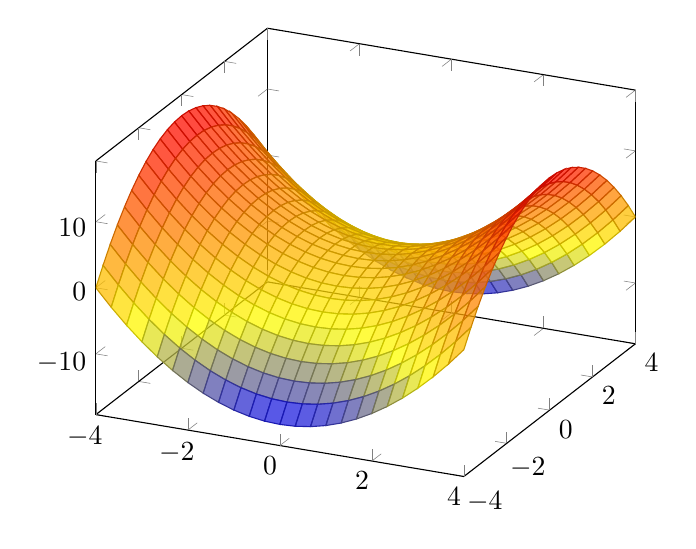
\begin{tikzpicture}
		\begin{axis}[view={25}{30},mark layer=like plot]
			\addplot3 [
				surf,
				shader=faceted,
				fill opacity=0.75,
				samples=25,
				domain=-4:4,
				y domain=-4:4,
				on layer=main,
			] {x^2-y^2};
		\end{axis}
	\end{tikzpicture}
	\caption{An example 3D plot done wit PGFplots.}
\end{figure}

And, of course the code for generating the plot is given as follows:

\begin{code}{latex}
\begin{figure}[!ht]
  \centering
  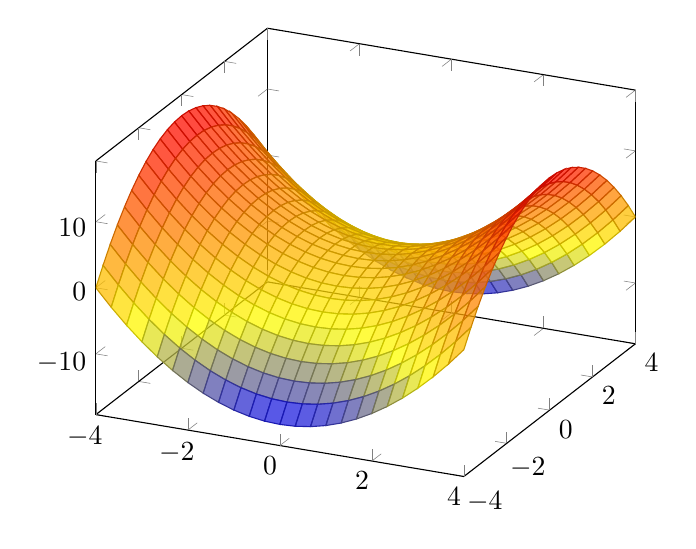
\begin{tikzpicture}
    \begin{axis}[view={25}{30},mark layer=like plot]
      \addplot3 [
      surf,
      shader=faceted,
      fill opacity=0.75,
      samples=25,
      domain=-4:4,
      y domain=-4:4,
      on layer=main,
      ] {x^2-y^2};
    \end{axis}
  \end{tikzpicture}
  \caption{An example 3D plot done wit PGFplots.}
\end{figure}
\end{code}

Some options worth mentioning are as follows:

\begin{hgitemize}
	\item[\pcode{surf}] Generates a \hlight{surface} based on the 2D
	data it was given (in this case these are $x$ and $y$.
	\item[\pcode{shader}] Describes, basically how each segment should be
	filled.
	\item[\pcode{samples}] Similar to 2D plots, tells how many data points will
	be measured. However, make a note that 3D is significantly more taxing
	on the TeX memory than 2D and making this sampling high may result in
	exceeding the memory limit.
\end{hgitemize}

\end{document}

%%% Local Variables:
%%% coding: utf-8
%%% mode: latex
%%% TeX-command-extra-options: "-shell-escape"
%%% TeX-master: t
%%% TeX-engine: luatex
%%% End:

